\documentclass[10pt]{beamer}

\usetheme{metropolis}
\usepackage{appendixnumberbeamer}

\usepackage{booktabs}
\usepackage[scale=2]{ccicons}

\usepackage{pgfplots}
\usepgfplotslibrary{dateplot}

\usepackage{xspace}
\usepackage{natbib}
\usepackage{blindtext}

\newcommand{\themename}{\textbf{\textsc{metropolis}}\xspace}

\title{Batik Classification using ConvNet and Transfer Learning}
\subtitle{Research progress report}
\date{\today}
\author{Yohanes Gultom - 1506706345}
\institute{IKO61181 Advance Image Processing}
% \titlegraphic{\hfill\includegraphics[height=1.5cm]{logo.pdf}}

\begin{document}

\maketitle

\begin{frame}{Table of contents}
  \setbeamertemplate{section in toc}[sections numbered]
  \tableofcontents[hideallsubsections]
\end{frame}

\section{Overview}

\begin{frame}{Research Proposal}

	\begin{itemize}[<+->]
		\item Batik image classification using ConvNet \cite{lecun2015deep}
		\item Using dataset from \cite{menzata2014sistem}
		\begin{itemize}
			\item 5 classes: Ceplok, Kawung, Lereng, Nitik, Parang
			\item 603 images			
		\end{itemize}
		\item Transfer learning from pre-trained VGG16 (ImageNet dataset) (\cite{simonyan2014very})
		\item Accuracy comparison with:
		\begin{enumerate}
			\item Convolutional stacked autoencoder (\cite{menzata2014sistem})
			\item Direct SIFT descriptor matching (\cite{willy2013evaluation})
		\end{enumerate}
	\end{itemize}

\end{frame}

\section{Methodology}

\begin{frame}{ConvNet by \cite{lecun2015deep}}

	\begin{figure}
		\centering
		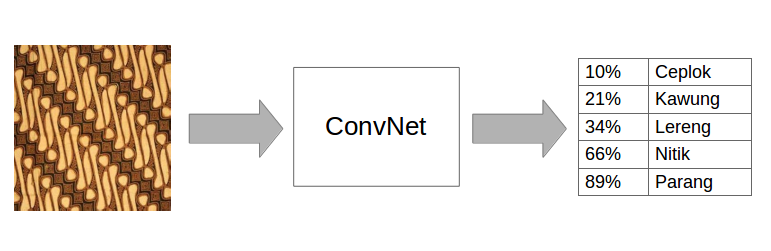
\includegraphics[width=1.0\linewidth]{convnet-batik}
		\caption{Classification with convolutional neural network}
		\label{fig_convnet_classification}
    \end{figure}

\end{frame}

\begin{frame}{ConvNet by \cite{lecun2015deep}}

	\begin{figure}
		\centering
		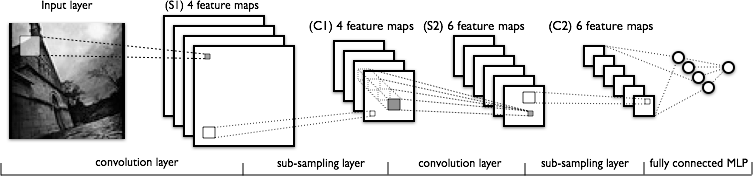
\includegraphics[width=1.0\linewidth]{lenet}
		\caption{Convolutional neural network (source: \url{deeplearning.net})}
		\label{fig_convnet}
    \end{figure}

\end{frame}

\begin{frame}{VGG16 by \cite{simonyan2014very}}

	\begin{figure}
		\centering
		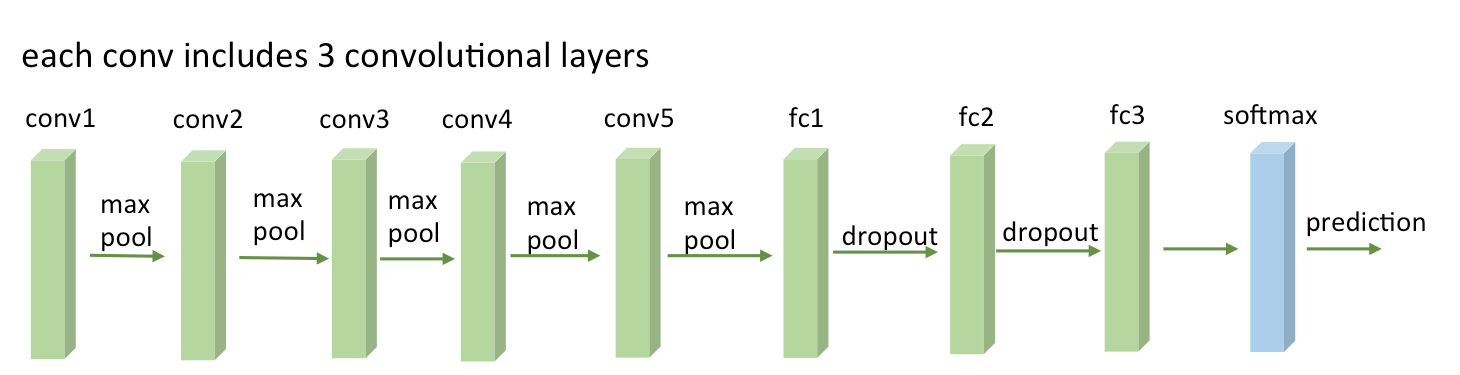
\includegraphics[width=1.0\linewidth]{vgg16arch}
		\caption{VGG-16 convnet (source: \url{sebastianraschka.com})}
		\label{fig_convnet_vgg16}
    \end{figure}

\end{frame}

\begin{frame}{Training Methods}

	\begin{enumerate}[<+->]
		\item Regular training
		\begin{itemize}
			\item Initialize convnet weights with zeros/random values
		\end{itemize}
		\item Transfer learning
		\begin{itemize}
			\item Initialize convnet weights with the weights of pretrained model (eg. VGG16 VGG19, ResNet50, Inception v3)
		\end{itemize}
	\end{enumerate}

\end{frame}

\section{Current Progress}

\begin{frame}{Transfer learning with VGG16}

	\begin{itemize}[<+->]
		\item Preprocessing
		\begin{itemize}
			\item Resize, vectorization \& normalization 603 images
		\end{itemize}
		\item Transfer learning
		\begin{itemize}
			\item VGG16 weight initialization
			\item Replace last layer with Softmax 5 output neurons
			\item Using stochastic gradient descent (SGD)
			\item Cross-validation using 9:1
			\item Only 5 epochs/iterations (12 hours onn CPU)
			\item Bad accuracy of 57\%
		\end{itemize}
		\item Using Python (OpenCV, Keras + Theano) \url{https://github.com/yohanesgultom/deep-learning-batik-classification}
	\end{itemize}

\end{frame}


\section{Remaining Works}

\begin{frame}{Remaining Works}

	\begin{itemize}[<+->]
		\item Increase data quantity by slicing images into patches
		\item Debug and tune architecture (increase epoch, adjust learning rate .etc)
		\item Do regular training (zero/random weights initialization)
		\item Run direct SIFT-descriptor matching on same data for comparison 
	\end{itemize}

\end{frame}

\begin{frame}[allowframebreaks]
  \bibliography{progress}
  %\bibliographystyle{abbrv}
  \bibliographystyle{plainnat}
\end{frame}

\begin{frame}[standout]
  Thank you
\end{frame}

\end{document}
